\section{Evaluation}\label{sec:evaluation}

In order to avoid over-fitting and be able to evaluate a real-world scenario for our trained model, the dataset is initially split into a \emph{training set} and a \emph{testing set}.
Consequently, every kind of consideration, analysis and training is made by using the training set only, to avoid information leaking from the testing set to the training set.

A powerful tool that can help us understand how to choose the most suitable regressor for each target value is the \emph{cross-validation}, explained in the following.
A final testing can be done at the very last stage, once we are satisfied with the result of the cross-validation and we are willing to test the obtained model against never seen data.

\subsection{Metrics}\label{sec:metrics}

In regression theory, there are two possible metrics that can be used to assess the accuracy of a regressor, which are different from the metrics used in classification theory, since the ground truth domain is continuous.

\paragraph{Mean Squared Error}
The MSE is a measure of the expected value of the quadratic error between each predicted value $y_i$ and its true value $\hat{y}_i$, therefore a lower value indicates a better accuracy.
Given $N$ as the number of samples, it is mathematically computed as follows:

\[
	\text{MSE}(y, \hat{y}) = \frac{1}{N} \sum_{i=1}^{N} (y_i - \hat{y}_i)^2
	\qquad [0, \infty)
\]

Since it is a scale-dependent metric, it is important to contextualize it into the scale of reference (i.e. a MSE of 0.2 is worse in a domain ranging from 1 to 10 than in one ranging from 1 to 100).

\paragraph{$R^2$-score}
The coefficient of determination is a measure of how well unseen samples are likely to be predicted by the model, and it represents the ratio between the variance of the predicted values and the variance that would be predicted by the model. Given $N$ as the number of samples, and $\bar{y}$ as the mean of the predicted values, it is mathematically computed as follows:

\[
	R^2(y, \hat{y}) = 1 - \frac{
		\sum_{i=1}^{N} (y_i - \hat{y}_i)^2
	}{
		\sum_{i=1}^{N} (y_i - \bar{y})^2
	} \qquad (-\infty, 1]
\]

It is a scale-invariant metric, therefore it is possible to compare $R^2$-scores across different domain ranges, however it is variance-dependent, so it might not be meaningful to compare it across different datasets.
A value of $1$ indicates that the regressor perfectly predicts the ground truth. A value of $0$ indicates that the regressor always predicts the mean value $\bar{y}$, disregarding the input features. A negative value indicates that the regressor behaves arbitrarily worse than predicting a constant.

\subsection{Cross-Validation}\label{sec:cross-validation}

It is a methodological error to evaluate metrics against the testing set and then use them to enhance the model, since this leaks information about the testing set which is supposed to be left unknown. This phenomenon is known as \emph{over-fitting} and should be avoided.

One possible option to evaluate the model without using the testing set is to cut a separate sub-set from the training set, called \emph{validation set}, and compute the metrics against this one instead. The drawback, however, is that this option further reduces the training set usable size.

A better approach consists in iteratively cutting a different small sub-set for validation from the training set, collect the metrics about each possible cut, and aggregate them in terms of mean and standard deviation (see figure~\ref{fig:kfolds}). This way, the whole training set can be used. This procedure is known as \emph{$k$-fold cross-validation}.

\begin{figure}
	\centering
	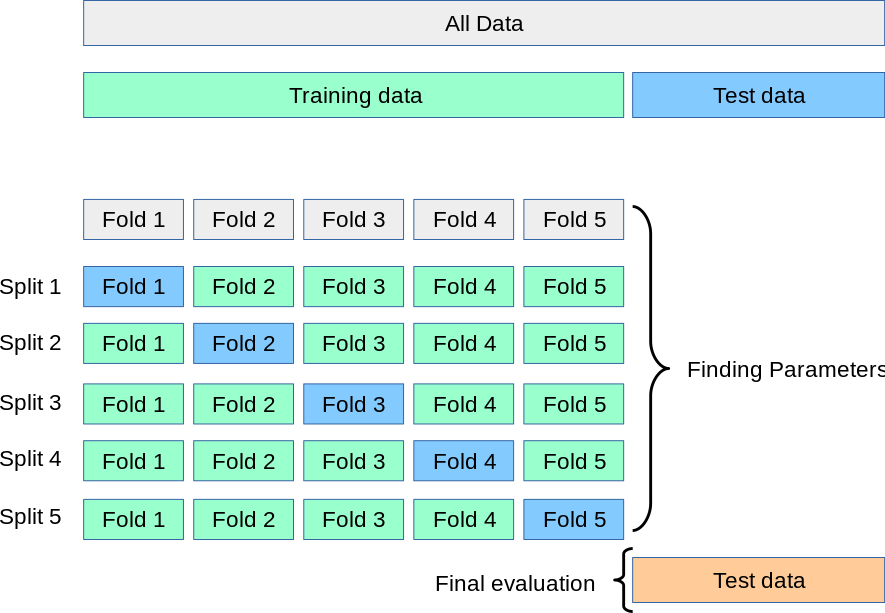
\includegraphics[width=0.5\linewidth]{assets/kfolds.png}
	\caption{$k$-fold cross-validation example with $k=5$ \cite{sklearn-crossval}}
	\label{fig:kfolds}
\end{figure}

The gathered metrics can effectively be used to evaluate the performance of the chosen regressors over the dataset. At this point, it is possible to tune the regression model (i.e. by changing the free parameters of the regressors) without the risk of over-fitting (see figure~\ref{fig:grid-search-workflow}).

\begin{figure}
	\centering
	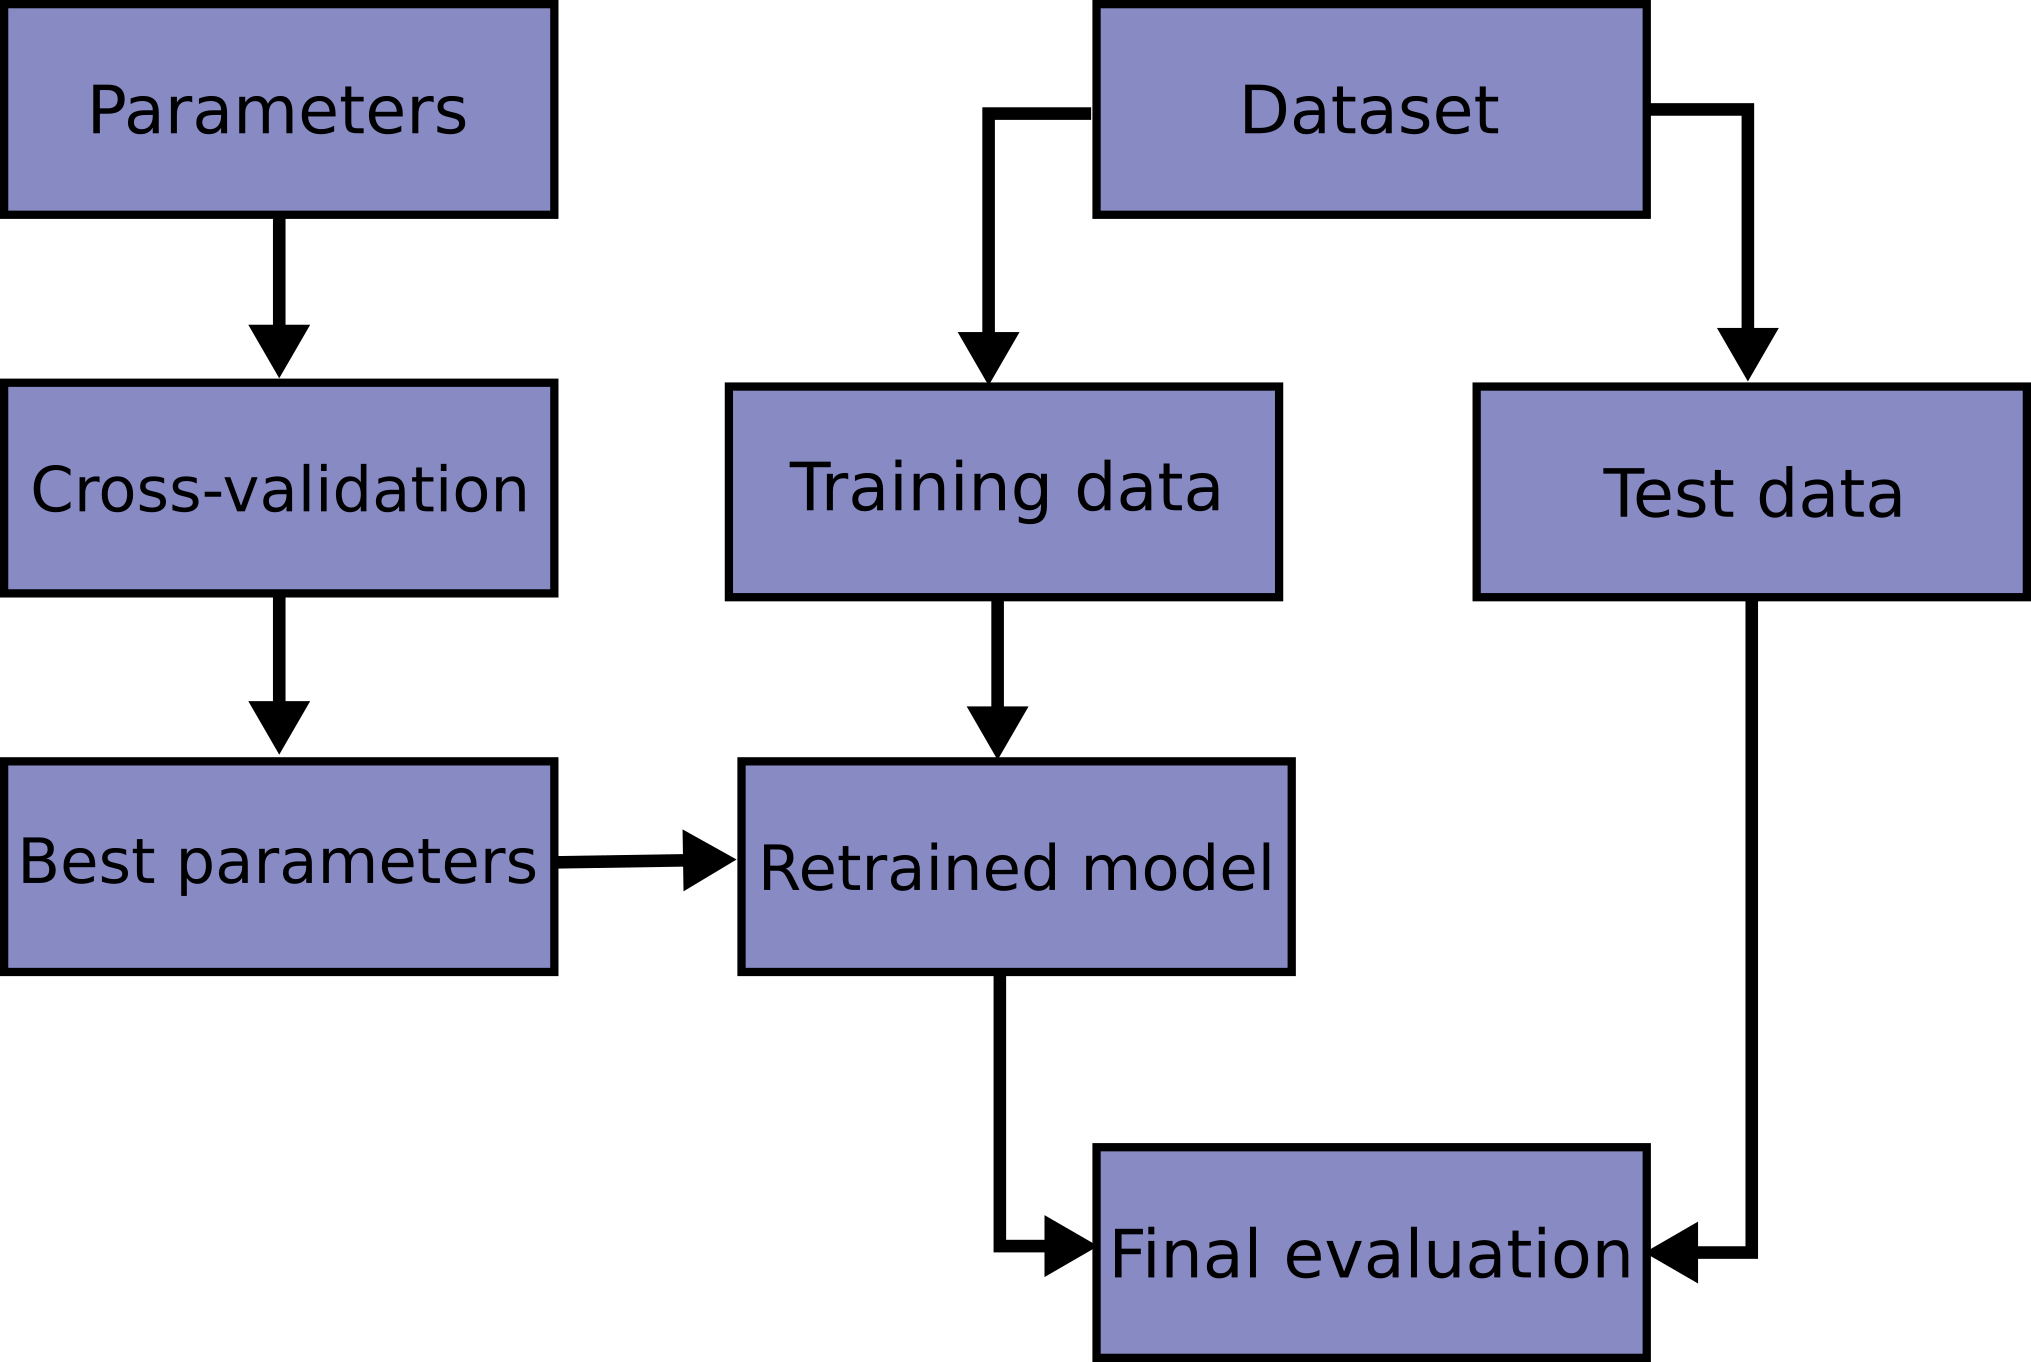
\includegraphics[width=0.5\linewidth]{assets/grid_search_workflow.png}
	\caption{Grid Search Workflow \cite{sklearn-crossval}}
	\label{fig:grid-search-workflow}
\end{figure}


\subsection{First tests}\label{sec:first-tests}

At first, we computed the scores of the 3 chosen regressors, \texttt{LinearRegression()}, \texttt{SVR()} and \texttt{KNeighborsRegressor(10, "distance")}, and we obtained the values in table~\ref{table:cross-scores}. It can be observed that, even after some kind of feature selection (both manual and automatic), no regressor could obtain a significant positive score for the values of "valence std" and "arousal std", which arises a problem on the dataset \todo{find a way to explain this part}.

\begin{table}
	\centering
	\begin{tabular}{lcccc}
		\toprule
		& valence mean & valence std & arousal mean & arousal std \\
		\midrule
		Linear & 0.46 ± 0.15 & -0.17 ± 0.17 & 0.45 ± 0.20 & -0.22 ± 0.53 \\
		SVR & 0.49 ± 0.11 & -0.02 ± 0.09 & 0.51 ± 0.13 & -0.06 ± 0.09 \\
		K-neighbors & 0.40 ± 0.08 & -0.06 ± 0.09 & 0.40 ± 0.16 & -0.07 ± 0.10 \\
		\bottomrule
	\end{tabular}
	\caption{Cross-validation $R^2$-scores with 95\,\% confidence intervals}
	\label{table:cross-scores}
\end{table}


\subsubsection{Automated cross-validation search}

The sklearn library provides a function \texttt{GridSearchCV()} for automatically selecting the best parameters for a given estimator, based on a grid of possible combinations.

\todo[inline]{una cross-validation vera con \texttt{GridSearchCV()} va fatta, altrimenti qui non possiamo scrivere nulla a riguardo}
